\documentclass[12pt, openany]{report}

\usepackage[T1]{fontenc}
\usepackage[utf8]{inputenc}
\usepackage[french]{babel}
\usepackage[a4paper,left=2cm,right=2cm,top=2cm,bottom=2cm]{geometry}

\usepackage{titlesec}
\usepackage{amssymb}
\usepackage{amsmath}
\usepackage{bm}
\usepackage{ulem}
\usepackage{bbold}
\usepackage{float}
\usepackage{libertine}
\usepackage[pdftex]{graphicx}
\usepackage[title,titletoc]{appendix}
\usepackage{textcomp}
\usepackage{gensymb}
\usepackage{newunicodechar}
\usepackage{caption}
\captionsetup{labelsep=space}
\usepackage{titlesec}
\usepackage{epsfig}
\usepackage{subcaption}
\usepackage{url}
\usepackage{hyperref}

\setlength{\parindent}{0cm}
\setlength{\parskip}{1ex plus 0.5ex minus 0.2ex}
\newcommand{\hsp}{\hspace{20pt}}
\newcommand{\HRule}{\rule{\linewidth}{0.5mm}}

\titleformat{\chapter}[hang]
  {\Huge\bfseries}{\thechapter{. }}{0pt}{\Huge}

\setcounter{tocdepth}{2}

\begin{document}

\begin{titlepage}
  \begin{sffamily}
  \begin{center}
    \HRule \\[0.4cm]
    { \huge \bfseries \textsc{3DFEM Python library}\\[0.4cm] }
    \HRule \\[0.5cm]
    
    \textsc{\Large User manual}\\[1cm]
    
    \textsc{\Large \bfseries To be added shortly}\\[1.8cm]
    
    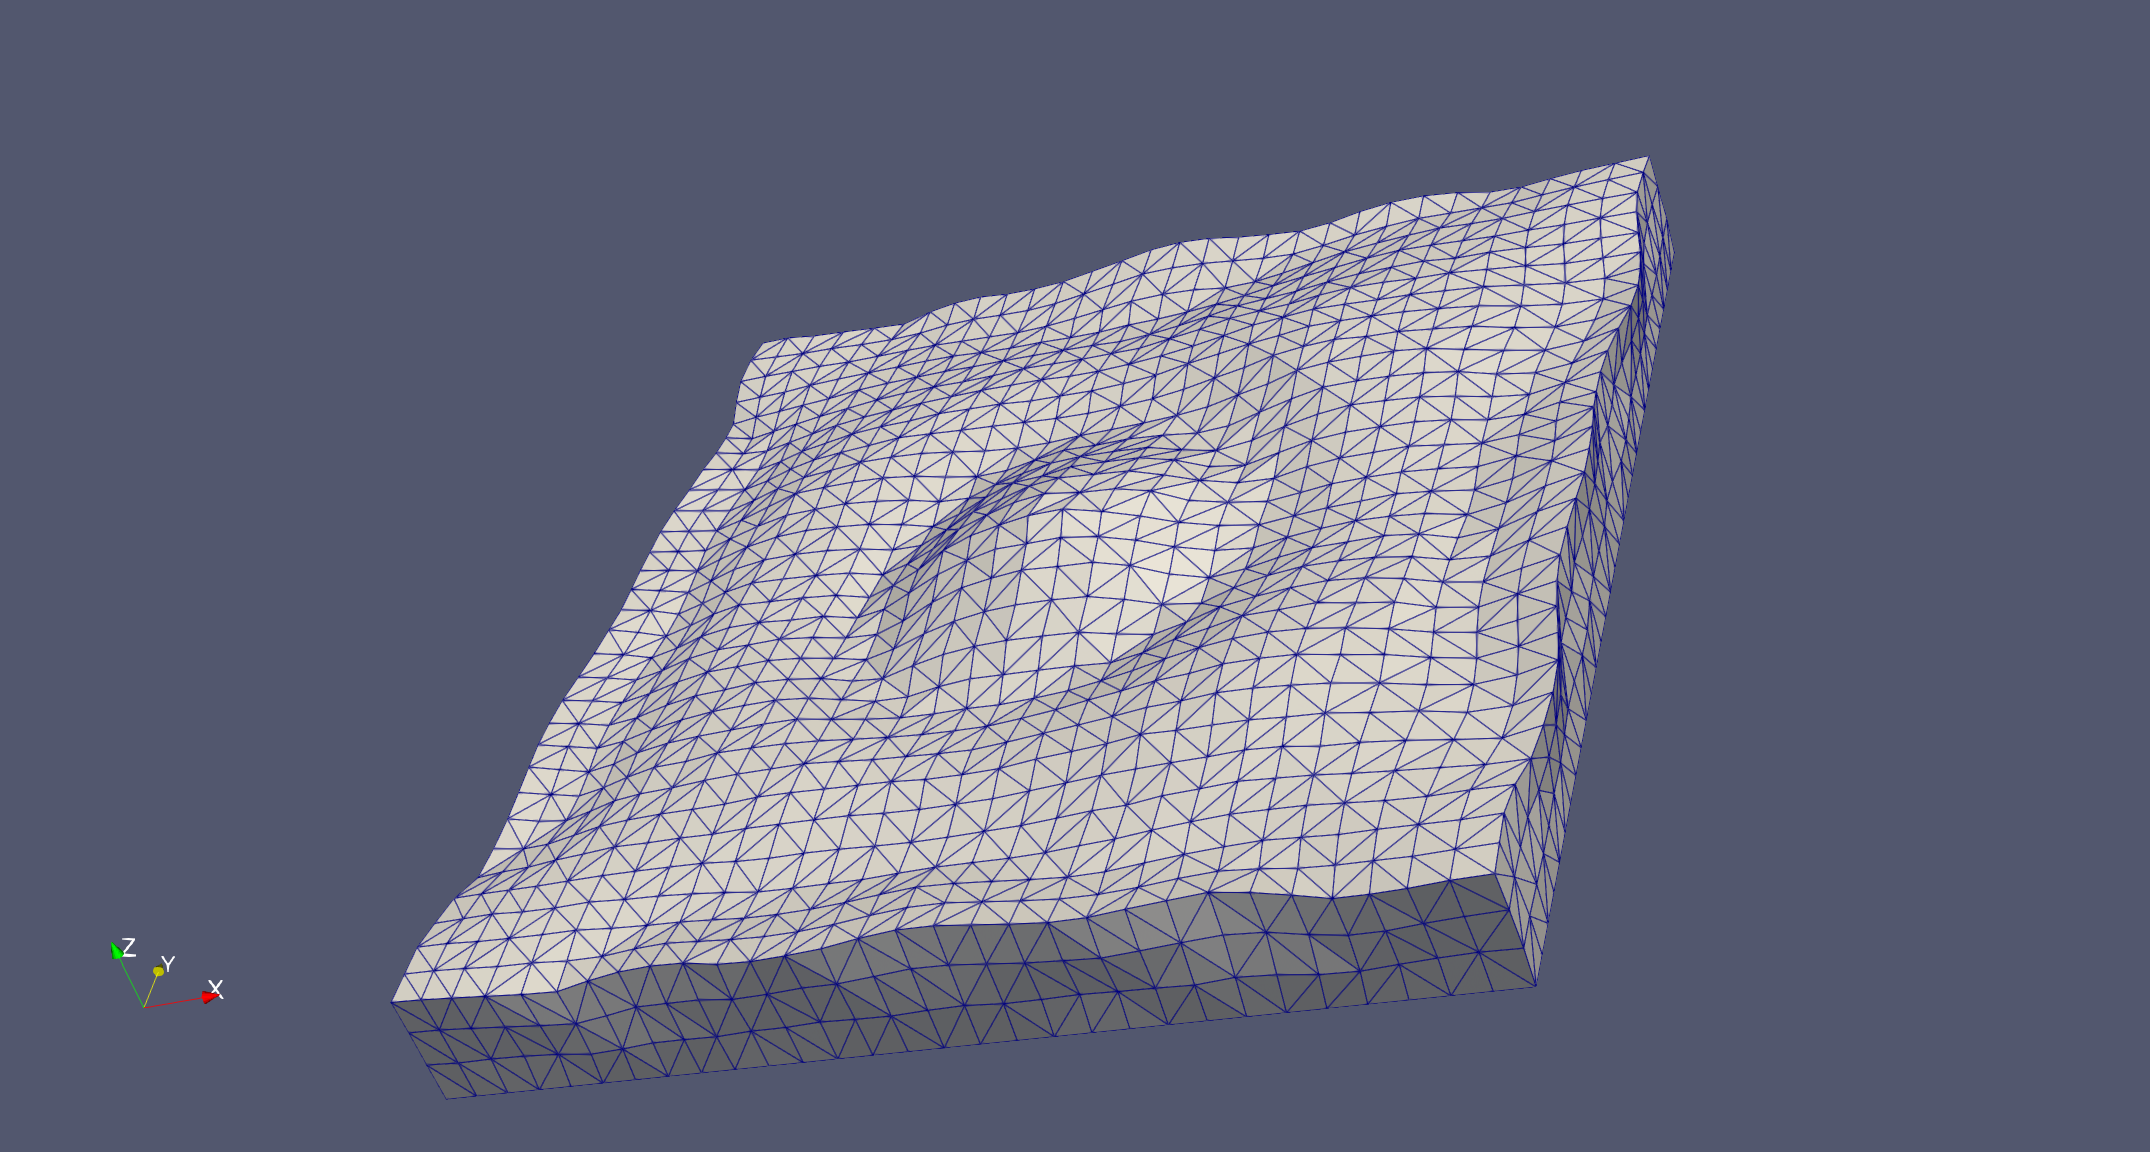
\includegraphics[scale=0.2]{3DFEM_image1.png}~\\[3cm]

    {\large \url{https://github.com/rcapillon/3DFEM}}\\[2cm]

    \begin{center}
    	\small Author: Rémi Capillon\\
    	\small \href{https://scholar.google.com/citations?user=q0jsk88AAAAJ}{Google Scholar page}\\
    \end{center}

    \vfill

    % Bottom of the page
    
  \end{center}
  \end{sffamily}
\end{titlepage}

% \tableofcontents

% \chapter{Manual}

\end{document}